\documentclass{beamer}
\usetheme{default}

\logo{
\includegraphics[width=.3in]{logo.png} \hspace{1em} Womprats T-16}
\title{ECE411 Final Presentation}
\subtitle{Womprats T-16 Audio Synthesizer}
\author{A. Goetz \and B. Kanyid \and J. Pugh \and K. Riedl}
\institute[PSU]{
  Maseeh College of Engineering and Computer Science\\
  Portland State University\\
  Portland, Oregon 97207  
}
\date{\today}


\begin{document}
\begin{frame}[plain]
  \titlepage
\end{frame}



% 30 seconds for overview
\section{Overview} 
\frame{{Project Overview} 
  \textit{What is the T-16 Audio Synth?}
  
  \pause A flexible Audio Synthesizer platform, capable of sweet
  riffs, and catchy hooks.  }


%\frame{\titlepage}
\frame{\frametitle{Agenda}\tableofcontents} 

\subsection{Objective}
\frame{{Objective}
  \textit{What is the objective of the T-16?}
\begin{itemize}
  \pause 
  \item Make Dead Week in the Capstone Lab as annoying as possible.

  \pause
  \item Demonstrate our ``Phat Engineering Skillz''

  \pause
  \item Develop an extensible music platform.

  \pause 
  \item Develop a project that is easy to demonstrate in an interview situation. 
\end{itemize}
}

\subsection{Requirements}
\frame{{Requirements}
\begin{itemize}
\item Avoid  mechanical complexity
\item Cheap to build
\item prefer inexpensive and open source tools
\item Gracefully degradeable
\item Breadboardable
\item Demonstratable in an interview situation
\end{itemize}
}

\subsection{Approach}
\frame{{Approach}
Project Management \& Documentation tools
\begin{itemize}
\item GanttProject
\item Redmine
\item \LaTeX and Beamer
\end{itemize}

Technical tools
\begin{itemize}
\item KiCad EDA
\item LPCXpresso Code Red IDE
\item Git
\end{itemize}
}

\section{Design}
\frame{\frametitle{Design}

	\centering
	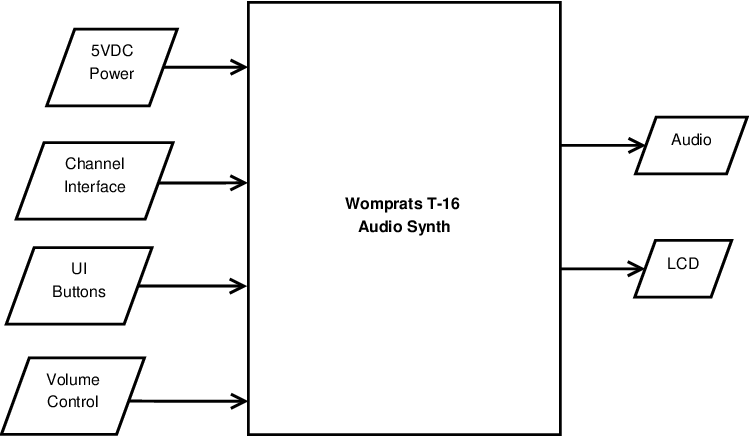
\includegraphics[width=0.7\textwidth]{synth0.png} 

}

\frame{\frametitle{Design}

	\centering
	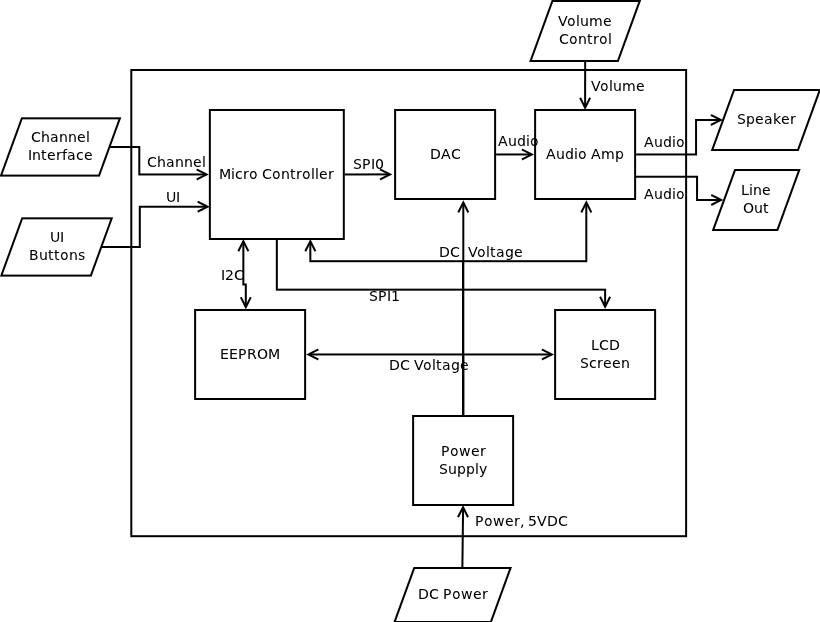
\includegraphics[width=0.7\textwidth]{synth1.png} 

}

\frame{\frametitle{Design}

	Microcontroller
	\begin{center}
	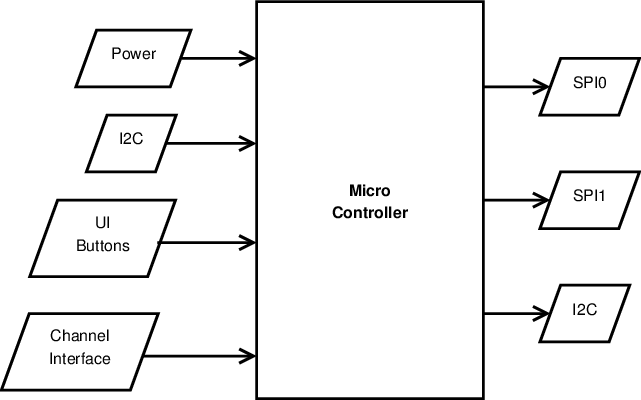
\includegraphics[width=0.6\textwidth]{microcont.png}
	\end{center}
	\begin{itemize}
	\item LPC1114 ARM microcontroller
	\item SPI and I$^2$C capable
	\item Multiple GPIO pins
	\item Simple, Cheap Dev Board (LPC Xpresso)
	\item Free development tools (code red)
	\item Available as DIP package to allow for prototyping
	\end{itemize}

}

\frame{\frametitle{Design}


	Channels 
        \begin{columns}
          \begin{column}{2in}
        \begin{itemize}
	\item 4 internal channels
		\begin{itemize}
		\item 4 internal channels
		\item 1 momentary switch for each
		\item 1 single turn pot for each
		\end{itemize}
	\item 2 external channels

		\begin{itemize}
		\item 1 port for each input
		\end{itemize}
	\item Output is voltage between 0V-3.3V
	\item Converted to 10-bit value by ADC in microcontroller
	\end{itemize}
        \end{column}
          \begin{column}{1in}
            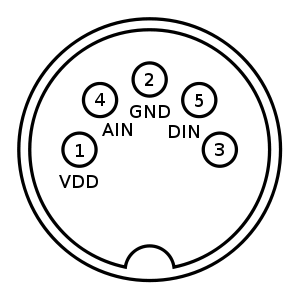
\includegraphics[width=1in]{mini-din.png}
            \end{column}
        \end{columns}

}

\frame{\frametitle{Design}
	UI \& LCD
	\begin{center}
	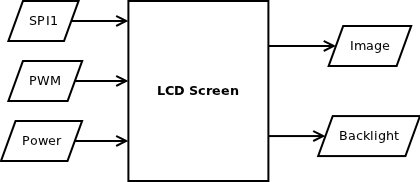
\includegraphics[width=0.7\textwidth]{lcd.png}
	\end{center}
	\begin{itemize}
	\item UI buttons
	\item channel buttons
	\item channel knobs
	\item LCD display
		\begin{itemize}
		\item EA DOGS102W-6 + EA LED39x41-W
		\end{itemize}
	\end{itemize}

}

\frame{\frametitle{Design}

	DAC \& Audio Out
	\begin{center}
	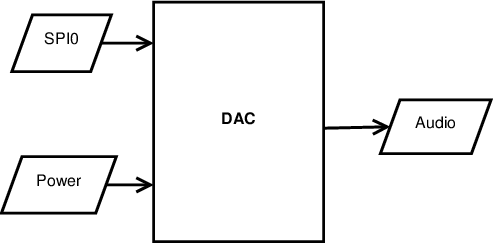
\includegraphics[width=0.5\textwidth]{dac.png}
	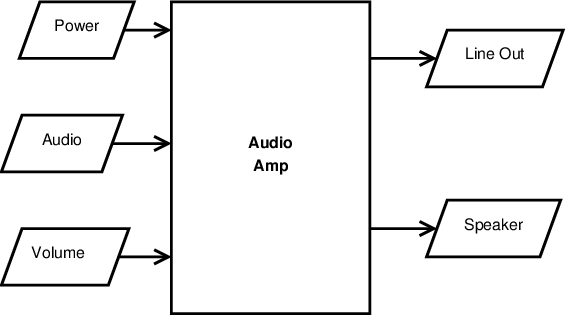
\includegraphics[width=0.5\textwidth]{audioamp.png}
	\end{center}
	\begin{itemize}
	\item 12-bit DAC
		\begin{itemize}
		\item SPI controlled
		\item Used MCP4921 DAC
		\end{itemize}
	\item Mono audio out
		\begin{itemize}
		\item LM4875 amplifier
		\end{itemize}
	\item Volume control
	\end{itemize}

}

\section{Implementation}
\frame{{Implementation}
  \begin{enumerate}
    \item Part Selection
    \item Prototyping
    \item Software Implementation
    \item Sunstone PCB
    \item Mechanical Design
  \end{enumerate}

}

\subsection{Part Selection}
\frame{{Part Selection}
  
}
\frame{{Microcontroller}
  \textbf{Selected Part: } NXP LPC1114
  \vfill
  \begin{columns}
    \column{2in}

  
    \textbf{Pros}
    \begin{itemize}
    \item Cheap Development Environment
    \item DIP Package
    \item Hardware Debugging
  \end{itemize}
  
  \textbf{Cons}
  \begin{itemize}
    \item Not as many examples as Atmel
    \item Closed source debugger
  \end{itemize}
  \column{2in}
  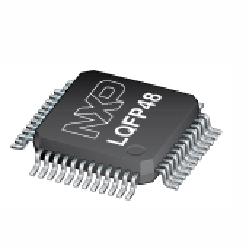
\includegraphics[width=1in]{lqfp.jpg}

  \end{columns}
}

\frame{{DAC}
    \textbf{Selected Part: } Microchip MCP4921
    \vfill
    \begin{columns}

    \begin{column}{1.5in}
    \textbf{Pros}
    \begin{itemize}
    \item Proven Design 
    \item DIP Package
    \end{itemize}
    
    \textbf{Cons}
    \begin{itemize}
    \item Complex SPI Interface
    \item Needs separate amplifier
    \end{itemize}
    \end{column}
    
    \begin{column}{1.5in}
      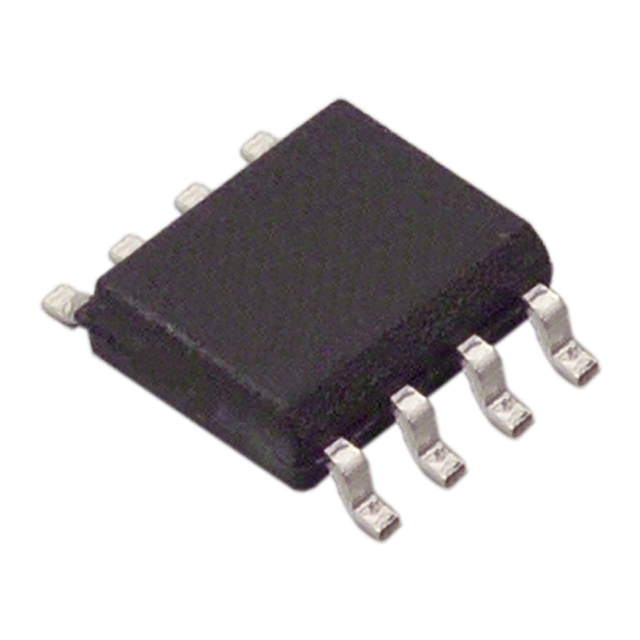
\includegraphics[width=1in]{soic.jpg}
    \end{column}
  \end{columns}
}

\subsection{Software}

\frame{\frametitle{Actual Board \& PCB}
\begin{center}
 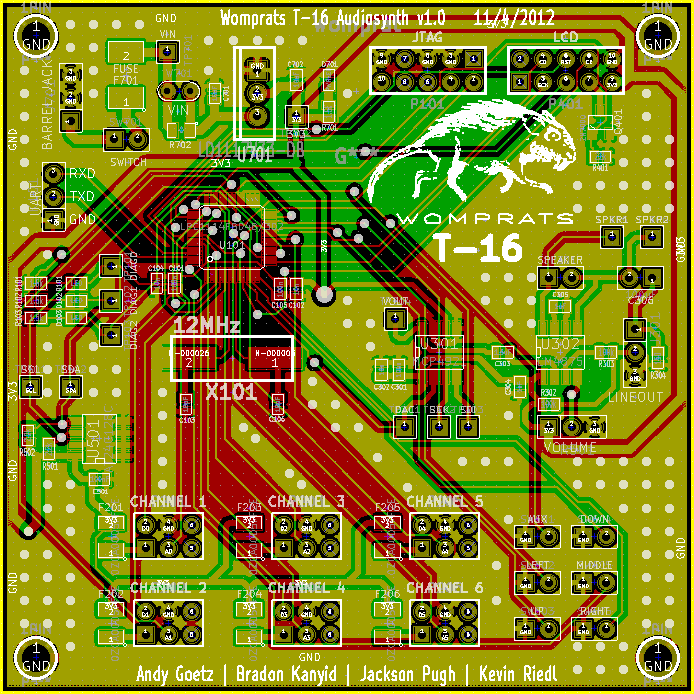
\includegraphics[width=0.45\textwidth]{pcb.png}
\end{center}
  Issue \#1: LDO pin layout incorrectly placed on the PCB\\
  Solution: Rotated LDO 180$^\circ$
}

\frame{\frametitle{Actual Board \& PCB}
\begin{center}
 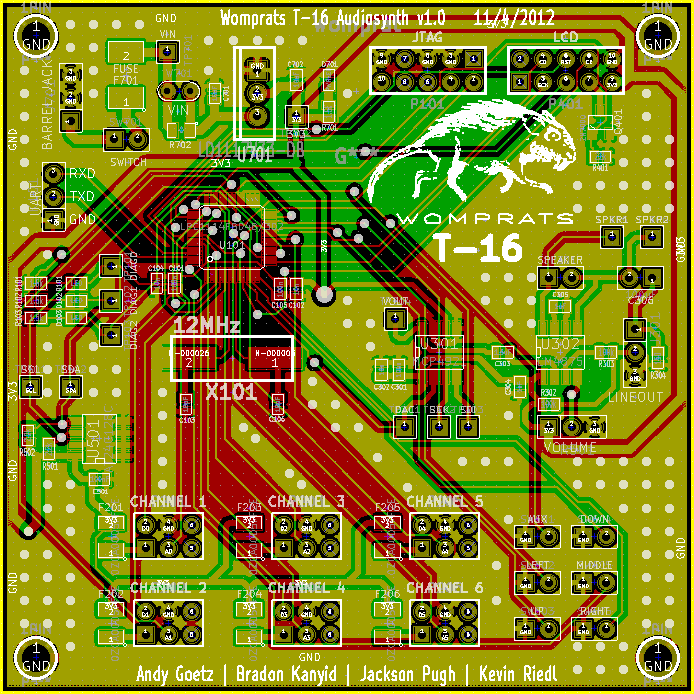
\includegraphics[width=0.45\textwidth]{pcb.png}
\end{center}
  Issue \#2: Unable to rapidly turn on and off the audio synthesizer\\
  Solution: Used pull-up resistor to force the bootloader pin high\\
}

\frame{\frametitle{Actual Board \& PCB}
\begin{center}
 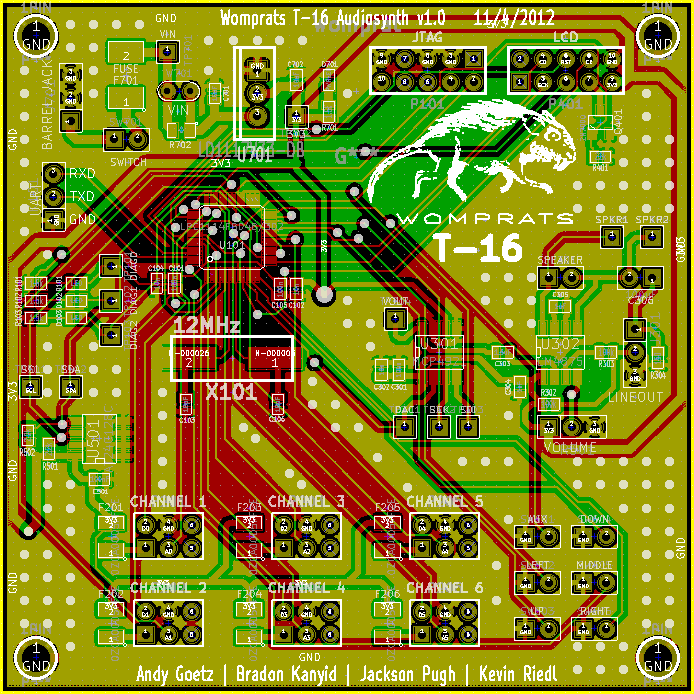
\includegraphics[width=0.45\textwidth]{pcb.png}
\end{center}
  Issue \#3: Header spacing width too close to fit together\\
  Solution: Shaved unnecessary header material to make it fit
}

\frame{\frametitle{Mechanical}
\begin{center}
 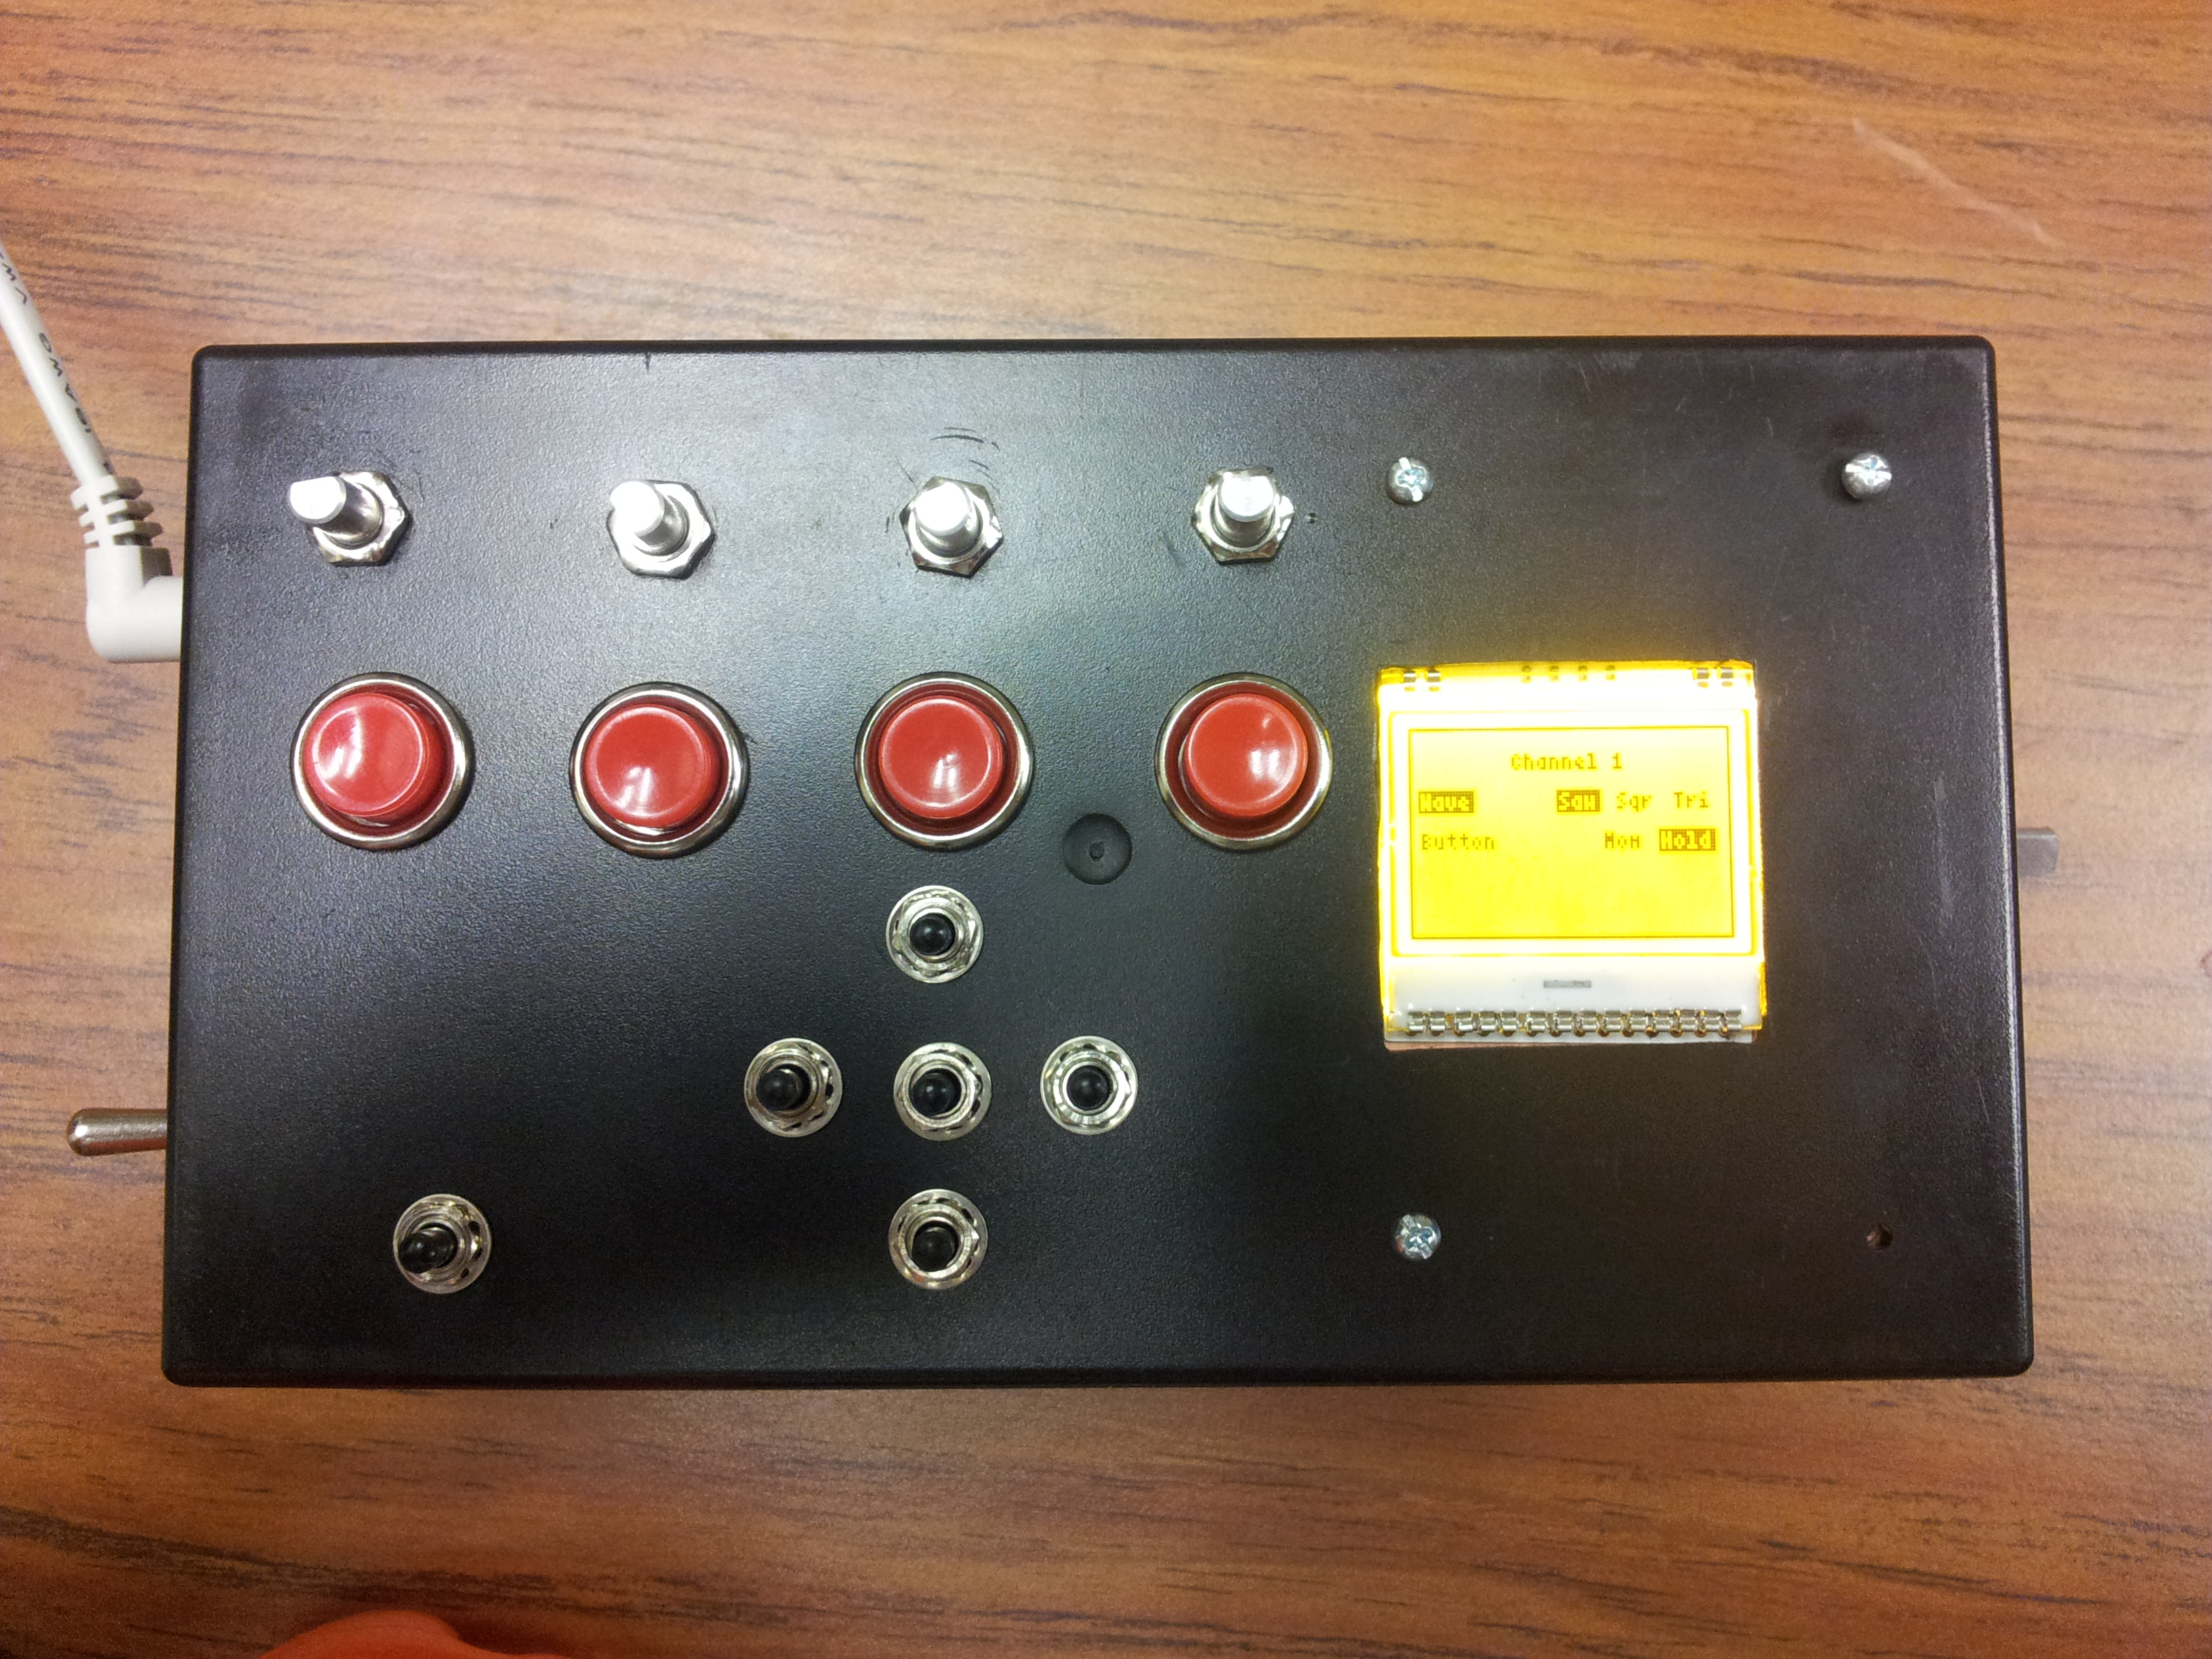
\includegraphics[width=0.5\textwidth]{unannotated.png}
\end{center}
}

\frame{\frametitle{BOM}
Insert finalized BOM table here:\\
}

\frame{\frametitle{IP/Prior Work}
\begin{itemize}
  \item LPCXpresso libraries for:
  \begin{itemize}
  \item Timers
  \item GPIO
  \item ADC
  \item SPI
  \item I$^2$C
  \end{itemize}
  \item Dogm128 LCD library (ported from ATmega)
  \item Bradon's Menu Code (written early 2000 for X)
\end{itemize}    
}

\subsection{PCB Layout}
\frame{{PCB Layout} 
}

\subsection{Implementation}

\frame{{Software}
\begin{itemize}
  \item LCD Core
  \begin{itemize}
    \item Display Womprat on Startup
  \end{itemize}
  \item Menu Core
  \begin{itemize}
    \item Display User Interface
  \end{itemize}
  \item Synth Core
\end{itemize}
}

\subsection{Implementation}
\frame{{Menu Core}
  \begin{center}
    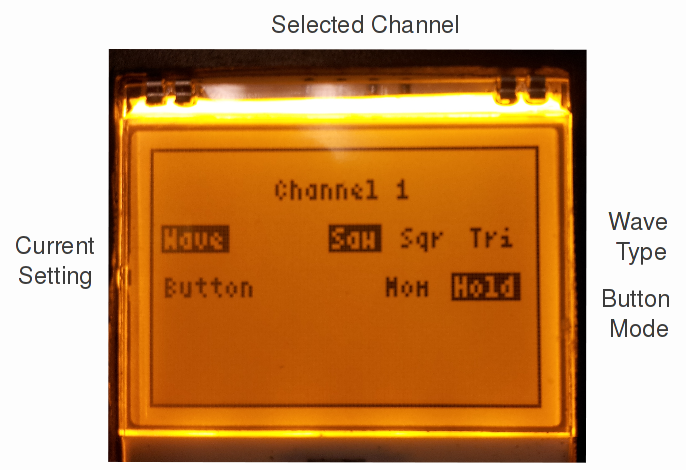
\includegraphics[width=0.7\textwidth]{LCD-annotated.png}
  \end{center}
  \begin{itemize}
    \item Select Waveform per Channel
      \begin{itemize}
      \item Sawtooth
      \item Square
      \item Triangle
    \end{itemize}
    \item Select Button Mode 
    \begin{itemize}
      \item Hold
      \item Momentary
    \end{itemize}
  \end{itemize}
}

\frame{{Synth Software}
  \begin{center}
    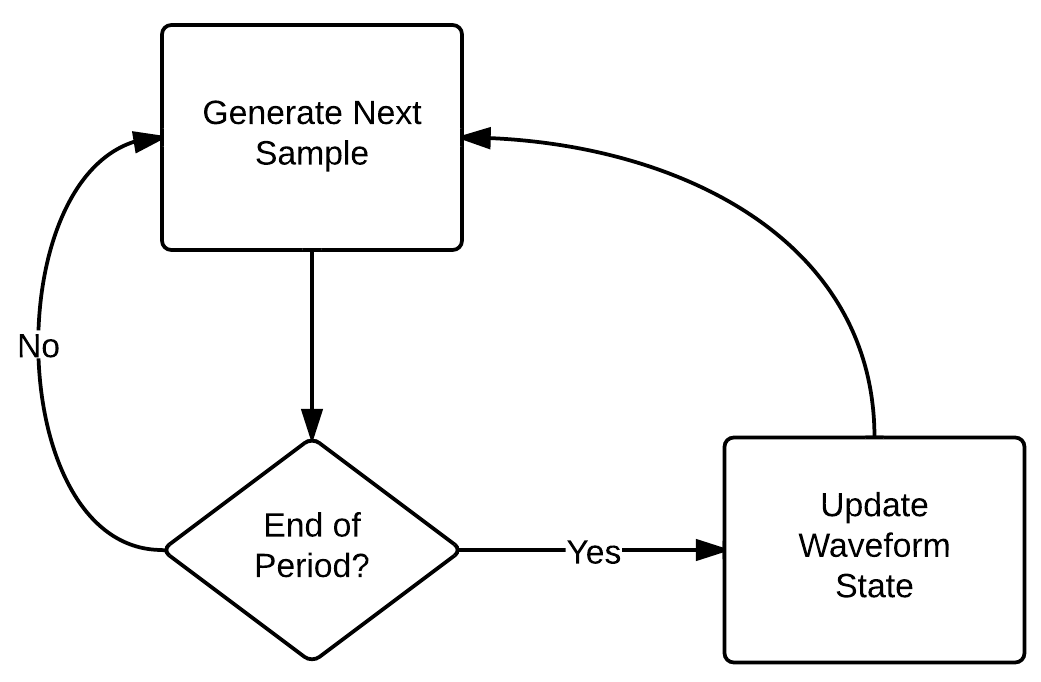
\includegraphics[width=3in]{synth-isr.png}
  \end{center}
  Broken down into three main parts: 
  \begin{itemize}
    \item Frequency Generation
    \item Waveform Generation
    \item Summing
    \end{itemize}

}

\frame{{Waveform Generation} 

  Generated Ramp functions are turned into Square, Sawtooth and
  Triangle waves using following transfer functions.
  
    \begin{columns}
    \begin{column}{1.1in}
      $f(x)$
      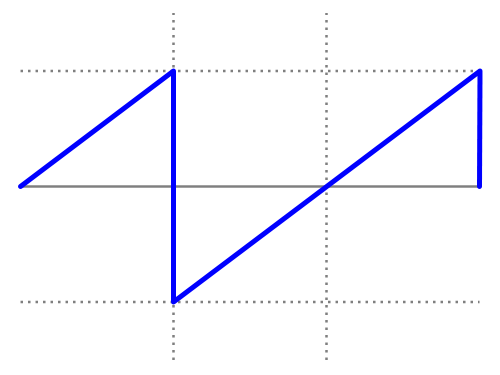
\includegraphics[width=1.4in]{sawtooth.png}
    \end{column}
    \begin{column}{1.9in}
      
      \begin{displaymath}
        f_{saw}(x) = 2f(x) - A
        \end{displaymath}
      
      \begin{displaymath}
        f_{squ}(x) = \left\{
        \begin{array}{lr}
          A & : x > A/2 \\
          -A & : x \le A/2
        \end{array}
        \right.
      \end{displaymath} 
      
      \begin{displaymath}
        f_{tri}(x) = \left\{
        \begin{array}{lr}
          4f(x) - A & : x \le A/2 \\
          -4f(x) + 3A & : x > A/2
        \end{array}
        \right.
      \end{displaymath} 
      

    \end{column}
  \end{columns}
}
\subsection{PCB Layout}
\frame{{PCB Layout} 
  \begin{center}
   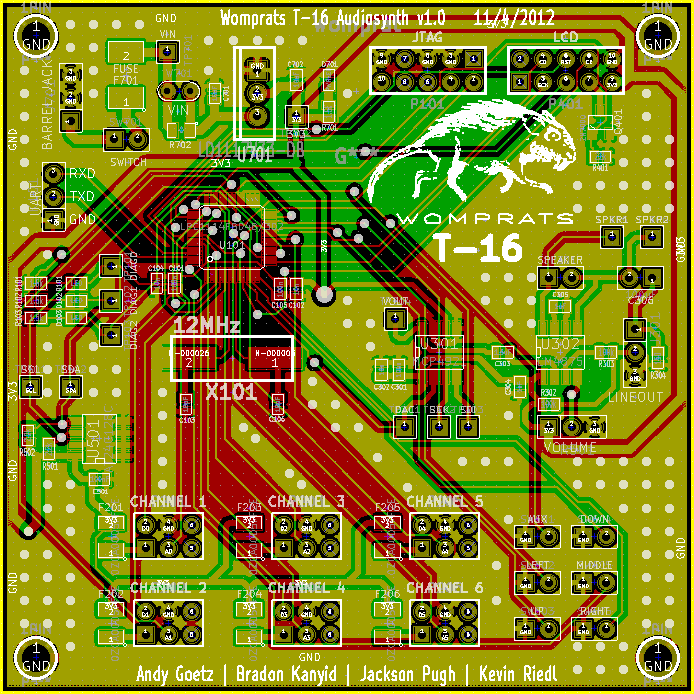
\includegraphics[width=0.7\textwidth]{pcb.png}
  \end{center}
}

\subsection{Testing}
\frame{{Testing}
\begin{itemize}
  \item Prototyping 
    \begin{itemize}
      \item Bottom up 
      \item Fast and Loose
      \item Unit testing was implicit 
    \end{itemize}
\end{itemize}
}

\subsection{Results}
\frame{{Results}
[Results text here]
}

\subsection{Contributions}
\frame{{Contributions}
[Contributions text here]
}
\subsection{Lessons Learned}
\frame{{Lessons Learned}
  \begin{itemize}
    \item Bradon Kanyid

    \item Andy Goetz

    \item Kevin Riedl

    \item Jackson Pugh
  \end{itemize}
}


%\section{Design Choices}
%\frame{\frametitle{Design Choices} 
%Design Choices text here
%}

%\begin{frame}{Design Choices}
%  \begin{itemize}
%    \pause
%  \item KiCad
%    \pause
%  \item LPC1114
%    \pause
%  \item GanttProject
%    \pause
%  \item \LaTeX
%    \end{itemize}
%\end{frame}



\end{document}
